\chapter{Fundamentos del algoritmo de Path Tracing}
	

En este capítulo se procede a dar un esquema básico de los fundamentos de este algoritmo. El objetivo será así describir un motor de renderizado previo a cualquier optimización, que cuenta con las funcionalidades básicas para producir una imagen de una escena tridimensional simple.

	\section{Aproximación de la ecuación de renderizado}
\[
{\displaystyle L_{\text{o}}(\mathbf {x} ,\omega _{\text{o}})=L_{\text{e}}(\mathbf {x} ,\omega _{\text{o}})\ +\int _{\Omega }f_{\text{r}}(\mathbf {x} ,\omega _{\text{i}},\omega _{\text{o}})L_{\text{i}}(\mathbf {x} ,\omega _{\text{i}})(\omega _{\text{i}}\cdot \mathbf {n} )\operatorname {d} \omega _{\text{i}}}
\]

La ecuación de renderizado \cite{kajiya1986rendering} aparece por primera vez en 1986 junto al algoritmo de Path Tracing, siendo este algoritmo una propuesta para resolverla. Es el pilar de la visualización 3d fotorrealista ya que simula de una manera suficientemente precisa la interacción de la luz en una escena tridimensional.

La interpretación de esta ecuación es la siguiente: Para un punto $\mathbf {x}$ del espacio y un ángulo $\omega _{\text{o}}$ desde el cual se observa a dicho punto, cuál es la cantidad de energía lumínica que el observador recibe $L_{\text{o}}$.

El primer término $L_{\text{e}}(\mathbf {x} ,\omega _{\text{o}})$ indica la luz que dicho punto $\mathbf {x}$ emite, así pues se podrán modelar materiales que emitan luz propia y no dependan de energía externa.

El segundo término calcula toda la luz entrante y reflejada a través del ángulo $\omega _{\text{o}}$ por dicho punto $\mathbf {x}$, es por ello que integra todos los ángulos del hemisferio superior. Este segundo término se compone de tres coeficientes:

El primer coeficiente $f_{\text{r}}(\mathbf {x} ,\omega _{\text{i}},\omega _{\text{o}})$ es la función BRDF, la cual es dependiente del material e indica cuánta energía se refleja en dicho punto para las direcciones de entrada $\omega _{\text{i}}$ y salida $\omega _{\text{o}}$.

El segundo coeficiente $L_{\text{i}}(\mathbf {x} ,\omega _{\text{i}})$ hace referencia a toda la energía lumínica entrante de todas las direcciones posibles.

El tercer coeficiente $(\omega _{\text{i}}\cdot \mathbf {n})$ es el producto de la ley del coseno de Lambert \cite{lambert1760jh}, un escalar que atenúa los ángulos menos pronunciados con la normal de la superficie.


	\section{Esquema simplificado del trazado de rayos}
	
Habiendo definido la ecuación de renderizado, el siguiente paso es explicar la implementación hecha de los fundamentos del algoritmo de Path Tracing, ya que posteriormente se irá mejorando paso por paso este algoritmo básico.

En su esencia consiste en trazar rayos o "caminos" desde una cámara virtual a una escena tridimensional, simulando así un modelo simplificado de fotones y sus interacciones con la escena. Tras cada interacción con la escena, estos caminos de fotones tienen una pérdida de energía que se acumulará en cada píxel y definirá el color de este, como si del sensor de una cámara real se tratara.

El primer paso es preparar la escena a renderizar \code{Scene}. Una escena básica se compone de una cámara \code{Camera}, geometrías \code{MeshObject} y materiales \code{Material}.

Las cámaras \code{Camera} consisten en una simulación aproximada de una cámara física real, así pues sus atributos serán: tamaño del sensor (en metros) \code{sensorWidth} y \code{sensorHeight}, distancia focal (en metros) \code{focalLength} y resolución (en píxeles) \code{xRes} e \code{yRes}. 

Las geometrías \code{MeshObject} por otra parte consisten en un conjunto de triángulos \code{Tri}, los cuales a su vez consisten en 3 puntos tridimensionales \code{Vector3 vertices[3]}.

Los materiales \code{Material} definen la manera en la que los fotones interactúan con ellos. En su forma más primitiva consisten en un color base, el cual absorberá ciertas longitudes de onda en mayor o menor medida. Para simplificar las computaciones, no es necesario calcular estas interacciones con todo el espectro electromagnético visible, basta con usar los tres colores primarios aditivos: rojo, verde y azul, así pues un color consiste en un vector \code{Vector3(R,G,B)}.

Habiendo definido estos elementos en la escena, se procederá a transferirlos a la GPU, donde se realizará el resto de computaciones más demandantes. Esto es realizado por la función \code{cudaError\_t renderSetup(Scene* scene)}, la cual a través de las funciones de la API de CUDA \code{cudaMalloc} y \code{cudaMemcpy} copia la información de la escena y lleva la cuenta de la memoria transferida en las variables globales \code{textureMemory, geometryMemory}. La copia de memoria de la CPU a la GPU requiere de un tratado especial para los objetos, requiriendo así una copia profunda de los atributos en formato array o punteros, además de un proceso posterior denominado "pointer binding".

%@todo explain pointerbinding
%@todo repharaphrasing and better organize this


\begin{figure}[H]
    \centering
	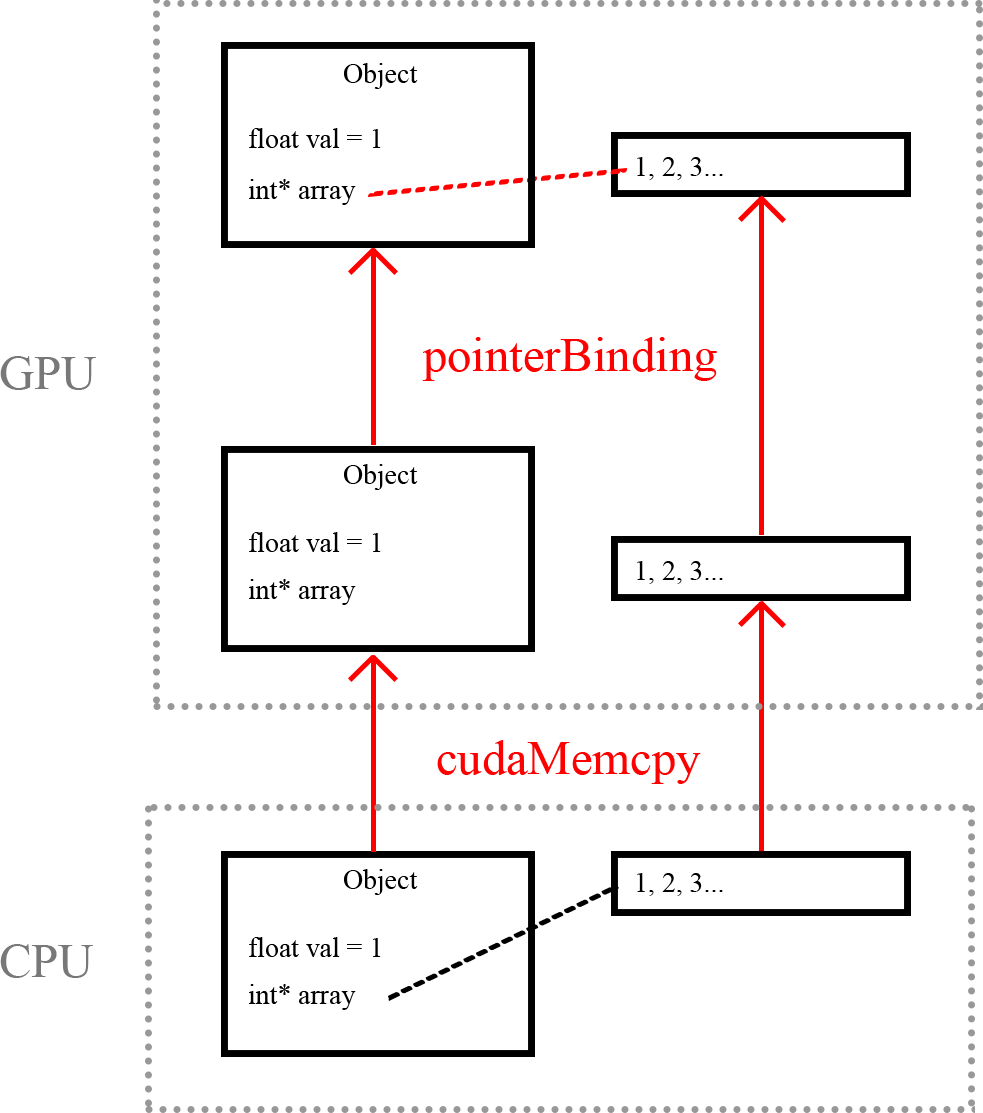
\includegraphics[width=0.5\textwidth]{pointerbinding}
	\caption{Pointer Binding}
	\label{fig:label}
\end{figure}

Una vez están todos los componentes necesarios en la GPU, es preciso llamar a un kernel para configurar el motor en la GPU. Este kernel \code{setupKernel} se hace cargo de inicializar los bufferes de píxeles y contador de rayos, inicializar \code{curand} (la librería utilizada para generar números aleatorios en CUDA) y por último asignar a cada objeto el índice de triángulos a l

%@todo improve setup kernel



	\subsection{Trazado de rayo desde la cámara}

Para simular el trazado del rayo desde la cámara hasta la escena, se simula de manera simplificada como funcionaría una cámara estenopéica. Se calcula la posición del sensor por la cual se trazará el rayo a partir de las coordenadas \code{x} e \code{y}. 

Puesto que no se está teniendo en cuenta la rotación de la cámara, la coordenada z del sensor se puede simplificar con la distancia de la cámara hasta el sensor.

\begin{lstlisting}
	
__device__ void calculateCameraRay(int x, int y, Camera& camera, Ray& ray, float r1, float r2) {

    // Relative coordinates for the point where the first ray will be launched
    float dx = camera.position.x + ((float)x) / ((float)camera.xRes) * camera.sensorWidth;
    float dy = camera.position.y + ((float)y) / ((float)camera.yRes) * camera.sensorHeight;

    // Absolute coordinates for the point where the first ray will be launched
    float odx = (-camera.sensorWidth / 2.0) + dx;
    float ody = (-camera.sensorHeight / 2.0) + dy;

    // Random part of the sampling offset so we get antialasing
    float rx = (1.0 / (float)camera.xRes) * (r1 - 0.5) * camera.sensorWidth;
    float ry = (1.0 / (float)camera.yRes) * (r2 - 0.5) * camera.sensorHeight;

    // Sensor point, the point where intersects the ray with the sensor
    float SPx = odx + rx;
    float SPy = ody + ry;
    float SPz = camera.position.z + camera.focalLength;

    // The initial ray is created from the camera position to the sensor point. No rotation is taken into account.
    ray = Ray(camera.position, Vector3(SPx, SPy, SPz) - camera.position);
}

\end{lstlisting}

	\subsection{Intersección triángulo - rayo}
	\label{subsec:triintersection}
	
El cálculo de la intersección de un rayo con un triángulo es una de las operaciones más fundamentales de este algoritmo. Esta operación toma como parámetros un triángulo \code{Tri} y un rayo \code{Ray} y ofrece como resultado si dicho triángulo y rayo intersectan en el espacio y además un objeto \code{Hit} el cual cuenta con información adicional de la intersección.

La información adicional que devuelve esta operación es la siguiente:

\begin{itemize}
	
	\item \code{int hit.objectID}: ID del objecto al que pertenece dicho triángulo.
	
	\item \code{Vector3 hit.position}: Posición en el espacio del punto de intersección entre el rayo y el triángulo.
	
	\item \code{Vector3 hit.normal}: Normal de la superficie, calculada a partir del producto vectorial de dos aristas del triángulo.
	
	\item \code{bool hit.valid}: Validez de una intersección, por defecto falso. Verdadero en caso de haber intersectado correctamente.

Para la implementación se ha hecho uso del algoritmo Fast Minimum Storage Ray/Triangle Intersection\cite{moller1997fast}. En este paper se explica detalladamente el algoritmo de intsersección, mientras este trabajo se limita a implementar dicho algoritmo a partir de una adaptación de la implementación en C que el autor ofrece.


\end{itemize}
	
\begin{lstlisting}
	
__host__ __device__ inline bool hit(Ray& ray, Hit& hit) {

float EPSILON = 0.0000001;

        Vector3 edge1 = vertices[1] - vertices[0];
        Vector3 edge2 = vertices[2] - vertices[0];

        Vector3 pvec = Vector3::cross(ray.direction, edge2);

        float u, v, t, inv_det;

        float det = Vector3::dot(edge1, pvec);

        inv_det = 1.0 / det;

        if (det > -EPSILON && det < EPSILON) return false;

        Vector3 tvec = ray.origin - vertices[0];

        u = Vector3::dot(tvec, pvec) * inv_det;
        if (u < 0.0 || u > 1.0)
            return false;

        Vector3 qvec = Vector3::cross(tvec, edge1);
        v = Vector3::dot(ray.direction, qvec) * inv_det;
        if (v < 0.0 || (u + v) > 1.0)
            return false;

        t = Vector3::dot(edge2, qvec) * inv_det;

        if (t < 0) return false;

        Vector3 geomPosition = ray.origin + ray.direction * t;
		Vector3 geomNormal = Vector3::cross(edge1, edge2).normalized();
		
		hit.normal = geomNormal;
		hit.position = geomPosition;
		hit.valid = true;
		hit.objectID = objectID;

        return true;

\end{lstlisting}

\section{Renderizado progresivo}
		
	Una ventaja de los motores de renderizado más modernos es el renderizado progresivo. Esto implica que las muestras se van acumulando poco a poco a lo largo de la imagen hasta que termina por converger. Esto difiere de los motores de renderizado por CPU tradicionales, que acumulan las muestras en secciones locales y una vez que acumulan las suficientes, pasan a la siguiente sección. Se ha decidido hacer una implementación progresiva con el fin de estar más cerca del estado del arte.
	
	Este tipo de implementación se beneficia de la copia de datos asíncrona de la GPU. Mientras el kernel se ejecuta, un flujo de datos secundario hará la copia del buffer de la GPU en la CPU, pudiendo así actualizar la visualización del resultado varias veces por segundo.

	Este flujo de datos secundario se ha implementado con el tipo de datos \code{cudastream\_t} de la API de CUDA. Han sido necesarios dos flujos, uno denominado \code{kernelStream} y otro denominado \code{bufferStream}. Los kernels de inicialización y renderizado correrán en el primero, mientras que la función que obtiene el buffer, será lanzada en el segundo.
	
	La función que extrae el buffer de píxeles de la GPU a la CPU es la siguente:
	
	\begin{lstlisting}
	cudaError_t getBuffer(float* pixelBuffer, int* pathcountBuffer, int size) {

		cudaStreamCreate(&bufferStream);

		cudaError_t cudaStatus = cudaMemcpyFromSymbolAsync(pixelBuffer, dev_buffer, size * sizeof(float) * 4, 0, cudaMemcpyDeviceToHost, bufferStream);
		if (cudaStatus != cudaSuccess) {
			fprintf(stderr, "returned error code %d after launching addKernel!\n", cudaStatus);
		}

		cudaStatus = cudaMemcpyFromSymbolAsync(pathcountBuffer, dev_pathcount, size * sizeof(unsigned int), 0, cudaMemcpyDeviceToHost, bufferStream);
		if (cudaStatus != cudaSuccess) {
			fprintf(stderr, "returned error code %d after launching addKernel!\n", cudaStatus);
		}

		return cudaStatus;
	}
	\end{lstlisting}
	
	Hace uso de la función \code{cudaMemcpyFromSymbolAsync} para realizar la copia asíncrona antes mencionada. También se hace copia del buffer de la suma de rayos emitidos por píxel con el fin de realizar métricas de eficiencia.
	
	%@todo analisis de movimiento de datos de memoria.


	










